% !TEX root = Index.tex
%Use Case-Diagramme und weitere \acs{UML}-Diagramme kann man auch direkt mit \LaTeX{} zeichnen, siehe \zB \url{http://metauml.sourceforge.net/old/usecase-diagram.html}.

\section{Anhang}

\subsection{Zeitplanung}
\label{app:timer}

\tabelle{Detaillierte Zeitplanung}{tab:Detaillierte Zeitplanung}{TimetableLong}

\subsection{Anwendung}
\label{app:useCase}

\subsubsection{Verwaltung von Diensten}
\label{app:useCase_controll}

\begin{center}
    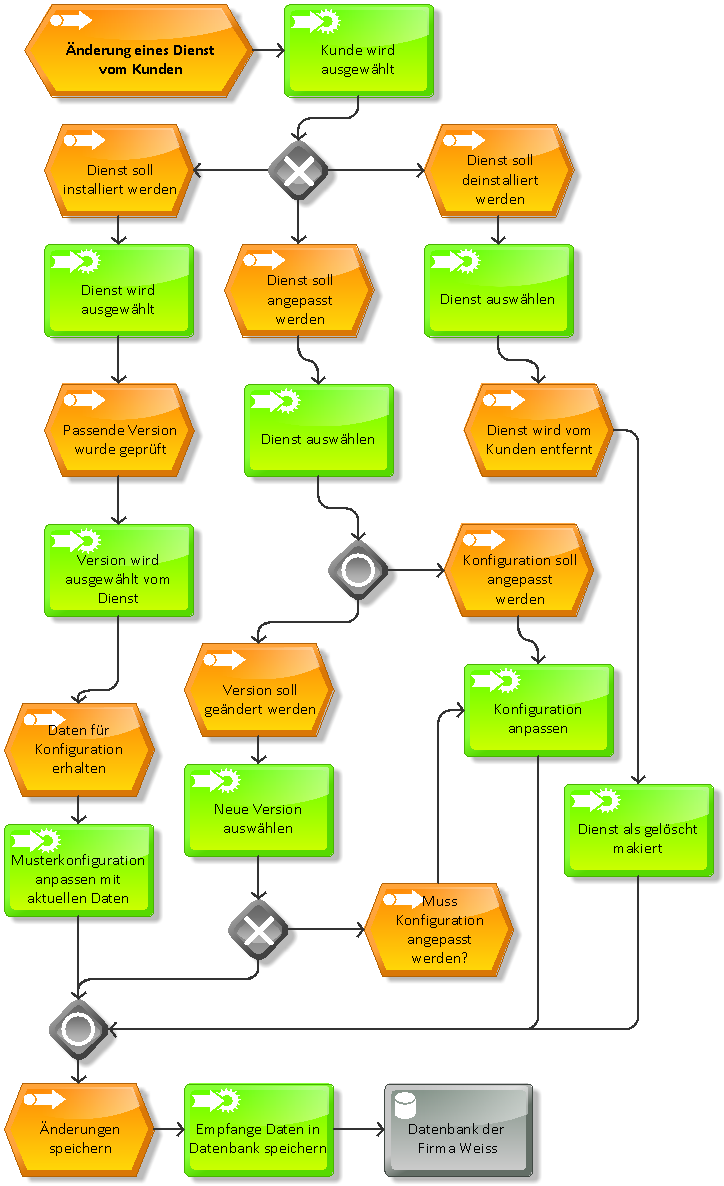
\includegraphics[scale=0.45]{content/attachments/GP_Service_Cltr.png}
\end{center}


\subsubsection{Dienstprüfung}
\label{app.useCase_check}

\begin{center}
    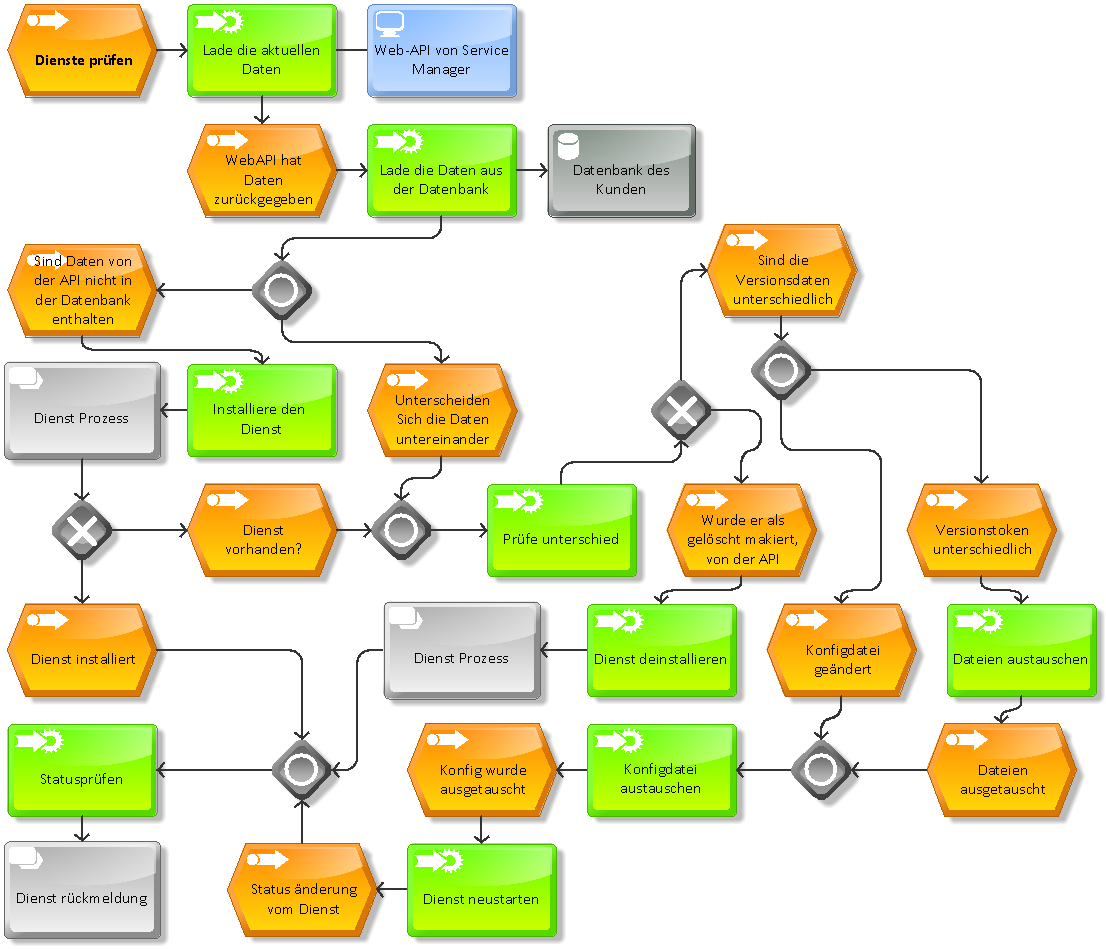
\includegraphics[scale=0.4]{content/attachments/GP_Service_Check.png}
\end{center}

\subsection{Oberfläche}
\label{app:view}

\subsubsection{Konzept}
\label{app:view_conc}

\begin{center}
    \begin{figure}[H]
        \centering
        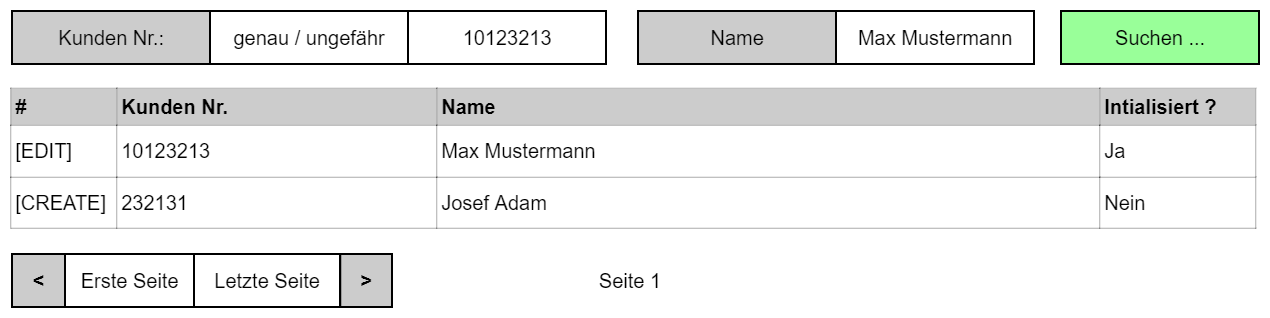
\includegraphics[scale=0.3]{content/attachments/k-cus-list.png}
        \caption{Kundenliste}
        \label{fig:k_cus_list}
    \end{figure}
    
    \begin{figure}[H]
        \centering
        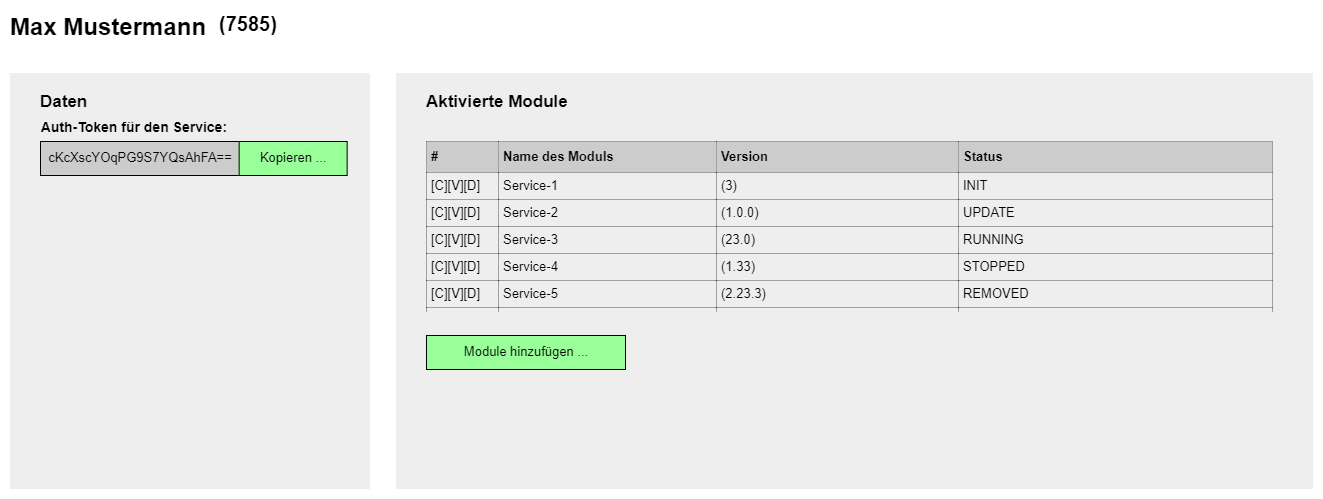
\includegraphics[scale=0.3]{content/attachments/k-cus-view.png}
        \caption{Kundenansicht}
        \label{fig:k_cus_view}
    \end{figure}
    
    \begin{figure}[H]
        \centering
        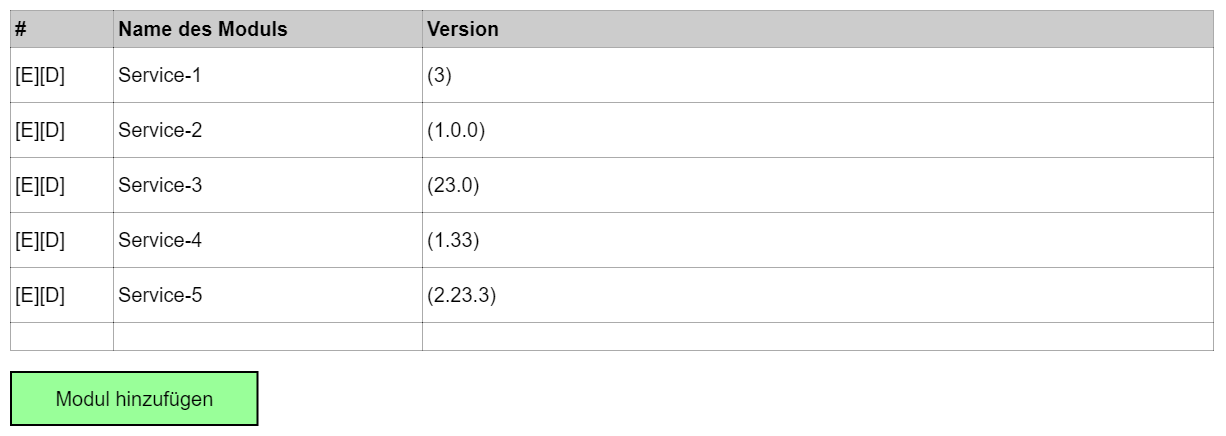
\includegraphics[scale=0.3]{content/attachments/k-ser-list.png}
        \caption{Dienstliste}
        \label{fig:k_ser_list}
    \end{figure}
    
    \begin{figure}[H]
        \centering
        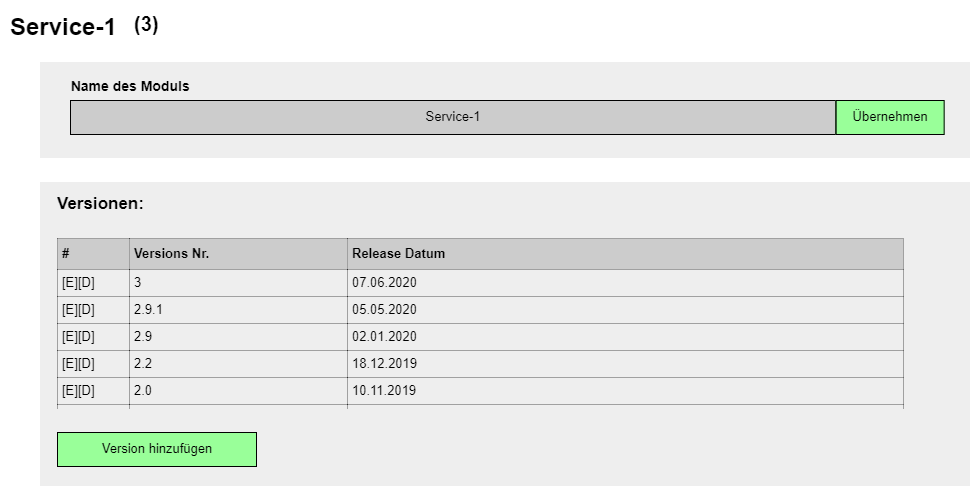
\includegraphics[scale=0.4]{content/attachments/k-ser-view.png}
        \caption{Dienstansicht}
        \label{fig:k_ser_view}
    \end{figure}
    
    \begin{figure}[H]
        \centering
        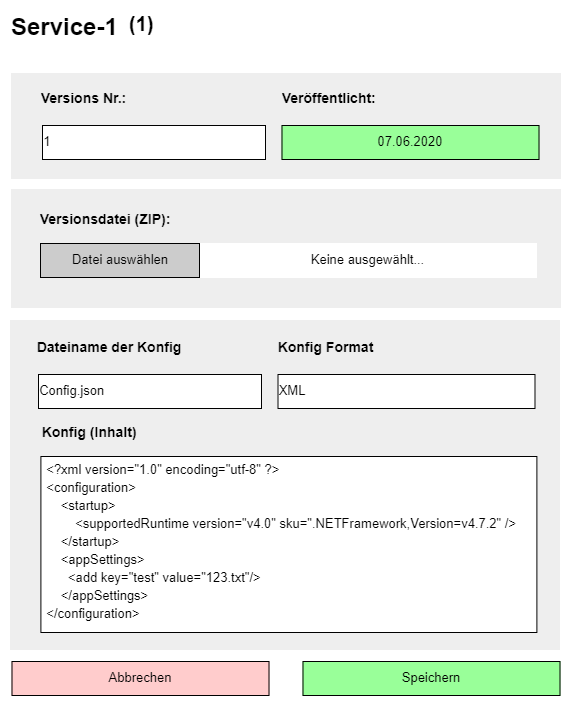
\includegraphics[scale=0.4]{content/attachments/k-ver-view.png}
        \caption{Versionseditor}
        \label{fig:k_ver_list}
    \end{figure}
\end{center}

\newpage

\subsubsection{Echtsystem}
\label{app:view_real}

\begin{center}
    \begin{figure}[H]
        \centering
        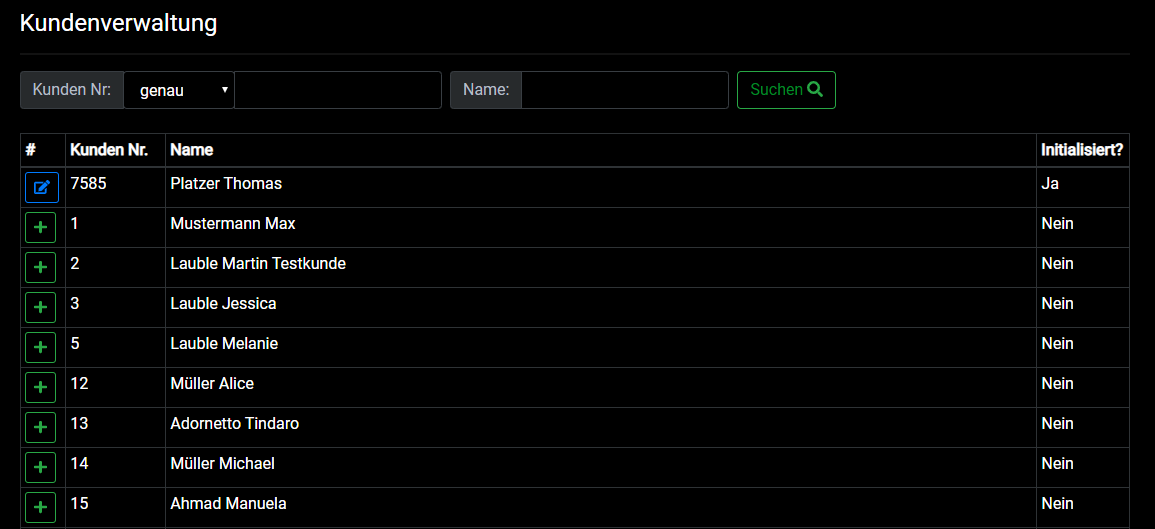
\includegraphics[scale=0.4]{content/attachments/s-cus-list.png}
        \caption{Kundenliste}
        \label{fig:s_cus_list}
    \end{figure}
    
    \begin{figure}[H]
        \centering
        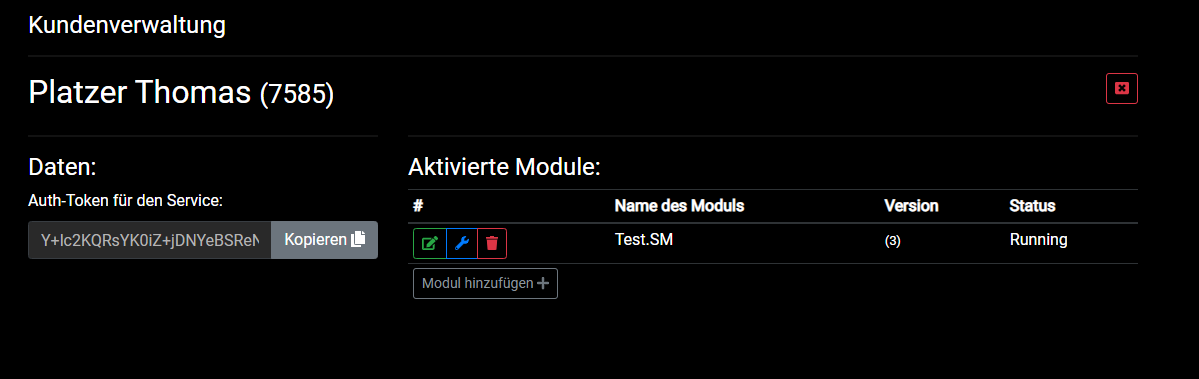
\includegraphics[scale=0.4]{content/attachments/s-cus-view.png}
        \caption{Kundenansicht}
        \label{fig:s_cus_view}
    \end{figure}
    
    \begin{figure}[H]
        \centering
        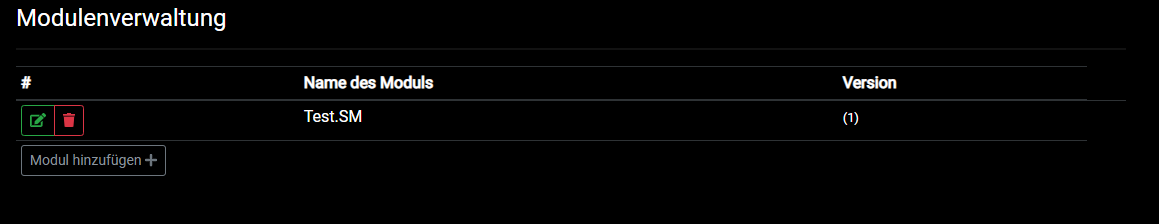
\includegraphics[scale=0.4]{content/attachments/s-ser-list.png}
        \caption{Dienstliste}
        \label{fig:s_ser_list}
    \end{figure}
    
    \begin{figure}[H]
        \centering
        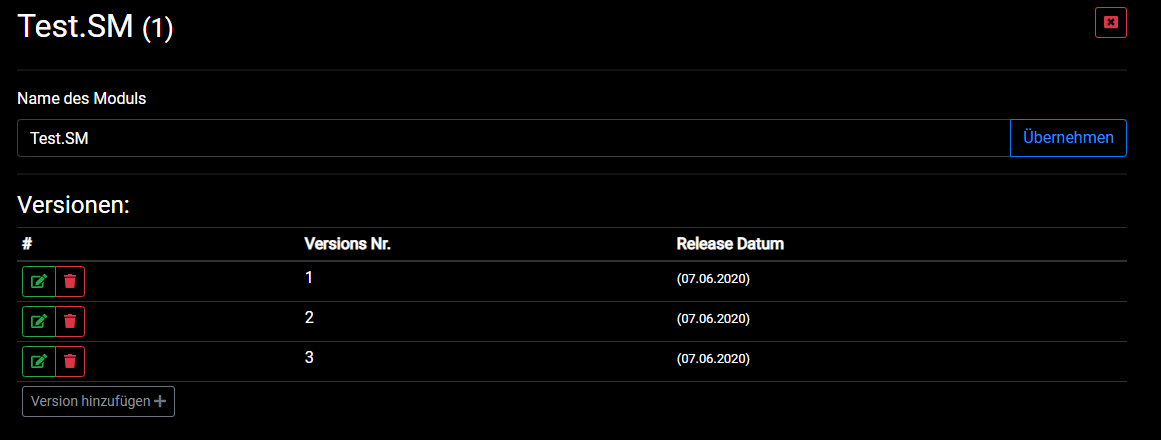
\includegraphics[scale=0.4]{content/attachments/s-ser-view.png}
        \caption{Dienstansicht}
        \label{fig:s_ser_view}
    \end{figure}
    
    \begin{figure}[H]
        \centering
        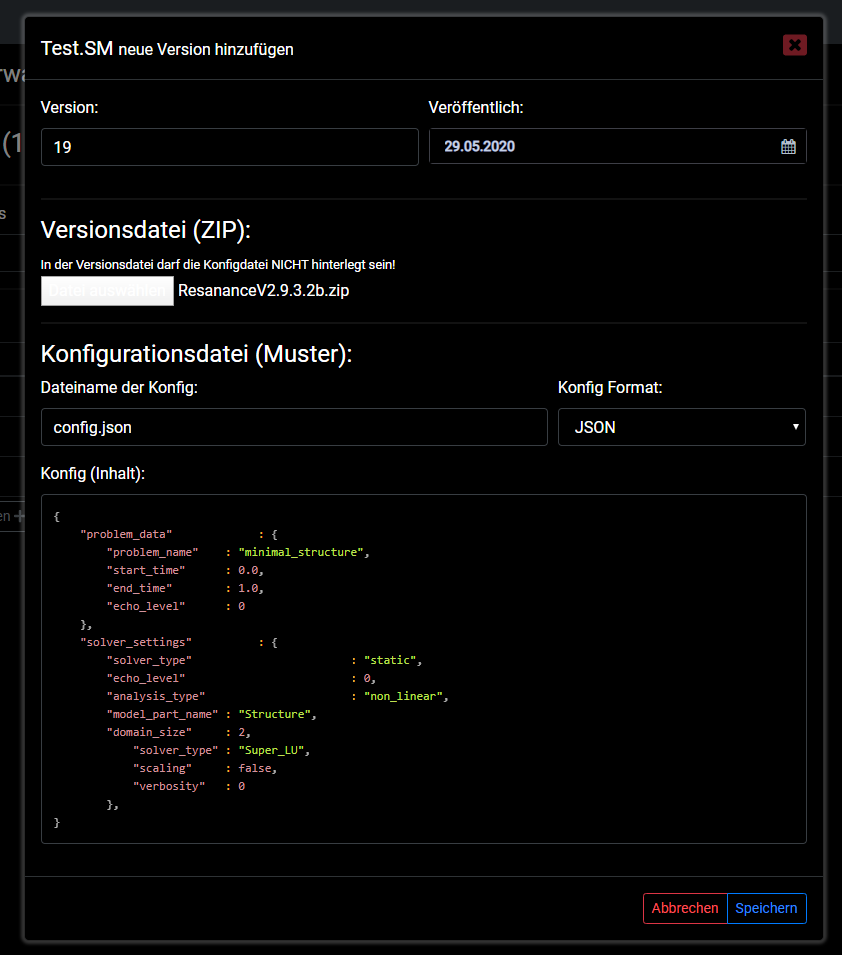
\includegraphics[scale=0.4]{content/attachments/s-ver-view.png}
        \caption{Versionseditor}
        \label{fig:s_ver_list}
    \end{figure}
\end{center}

\subsection{Klassendiagramme}
\label{app:class_concept}

\begin{center}
    \begin{figure}[H]
        \centering
        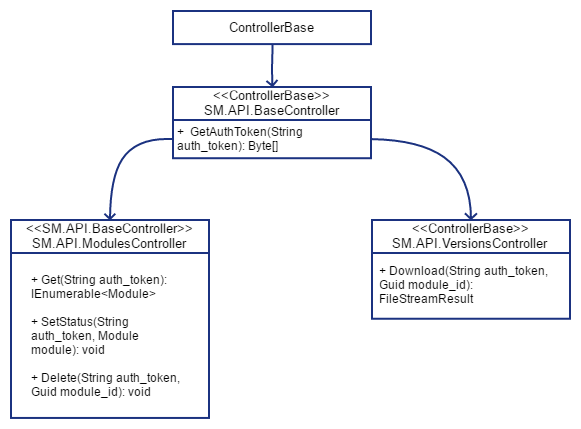
\includegraphics[scale=0.4]{content/attachments/c-api-cntrl.png}
        \caption{Controller-Klassen der API Anwendung}
        \label{fig:c-api-cntrl}
    \end{figure}
    
    \begin{figure}[H]
        \centering
        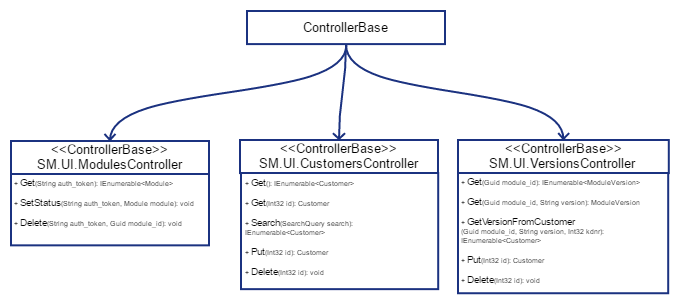
\includegraphics[scale=0.4]{content/attachments/c-ui-cntrl.png}
        \caption{Controller-Klassen der Oberflächen/UI Anwendung}
        \label{fig:s_cus_view}
    \end{figure}
\end{center}

\subsection{Tabellenmodell}
\label{app:database_table}

\begin{center}
    \begin{figure}[H]
        \centering
        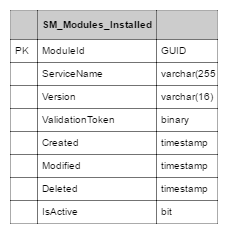
\includegraphics[scale=0.4]{content/attachments/d-table-cus.png}
        \caption{Tabelle die in der Kunden-Datenbank ist}
        \label{fig:d-table-cus}
    \end{figure}
    
    \begin{figure}[H]
        \centering
        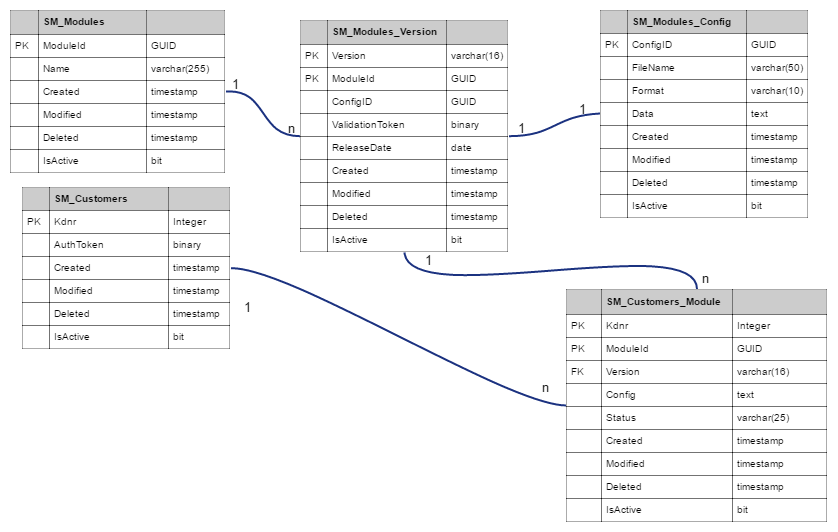
\includegraphics[scale=0.4]{content/attachments/d-table-wss.png}
        \caption{Tabellen in der Datenbank der Firma Weiss}
        \label{fig:d-table-wsss}
    \end{figure}
\end{center}

\subsection{Quellcode}
\label{app:sourceCode}

\begin{center}
 \lstinputlisting
    [caption={Quellcode zum importieren der Funktionen, um Dienste verwalten zu können}
       \label{lst:import-cs},
       captionpos=t,language=CS]
 {content/code/p-import.cs}
 
 \lstinputlisting
    [caption={Quellcode um Dienste installieren zu können (DLLs müssen importiert sein!)}
       \label{lst:install-cs},
       captionpos=t,language=CS]
 {content/code/p-install.cs}
 
 \lstinputlisting
    [caption={Quellcode zum entfernen der Dienste (DLLs müssen importiert sein!)}
       \label{lst:delete-cs},
       captionpos=t,language=CS]
 {content/code/p-delete.cs}
\end{center}